\chapter{}

\begin{figure}[h]
\centering
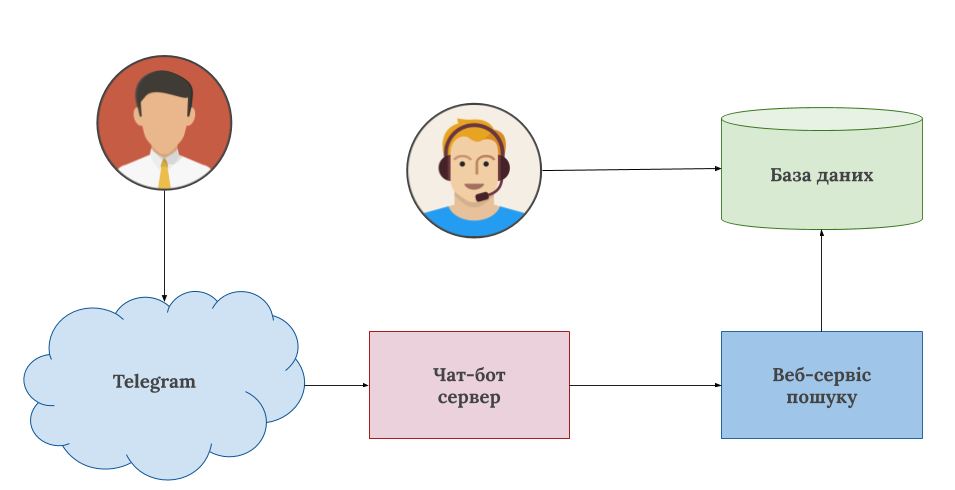
\includegraphics[width=0.5\textwidth]{user-system-overview}
\caption{Схема роботи користувацької системи}
\label{fig:user-system-overview}
\end{figure}

\begin{figure}[h]
\centering
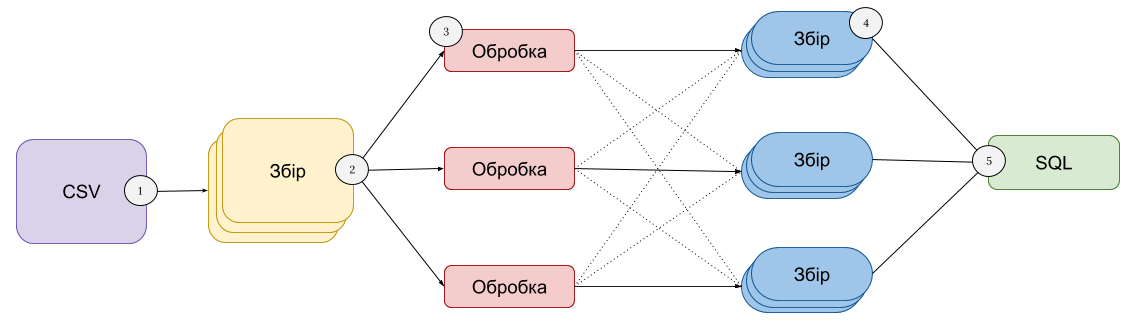
\includegraphics[width=0.7\textwidth]{parser-overview}
\caption{Обробка документів формату CSV у SQL}
\label{fig:parser-overview}
\end{figure}

\begin{figure}[h]
\centering
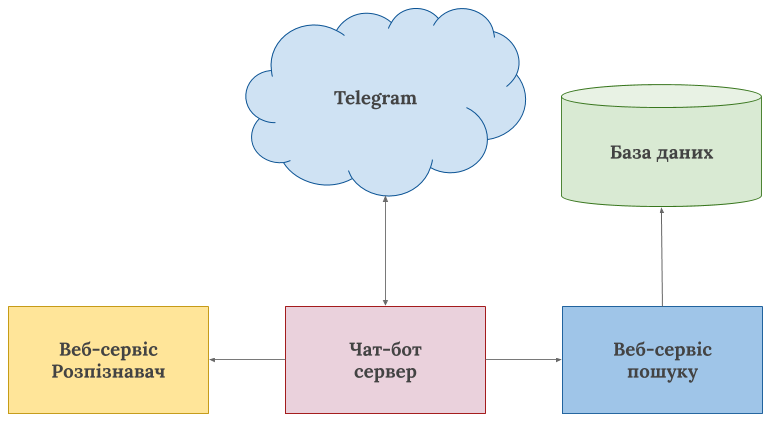
\includegraphics[width=0.5\textwidth]{architecture-overview}
\caption{Повна схема роботи системи}
\label{fig:architecture-overview}
\end{figure}

\pagebreak

\begin{lstlisting}[caption={Реалізація функції Map.},captionpos=b]
func mapper(input chan []string, output chan model.Operation) {
	for {
		msg, opened := <- input
		if !opened {
			return
		}

		output <- *model.NewOperation(msg)
	}
}
\end{lstlisting}

\begin{lstlisting}[caption={Реалізація функції Reduce.},captionpos=b]
func reducer(input chan []model.Operation, output chan struct{}) {
	db := database.Must(database.DB())
	defer db.Close()

	for {
		operations, open := <-input
		if !open {
			output <- struct{}{}
			return
		}

		if err := db.Insert(&operations); err != nil {
			// Handle error.
		}
	}
}
\end{lstlisting}
